\begin{figure}
  \begin{center}
  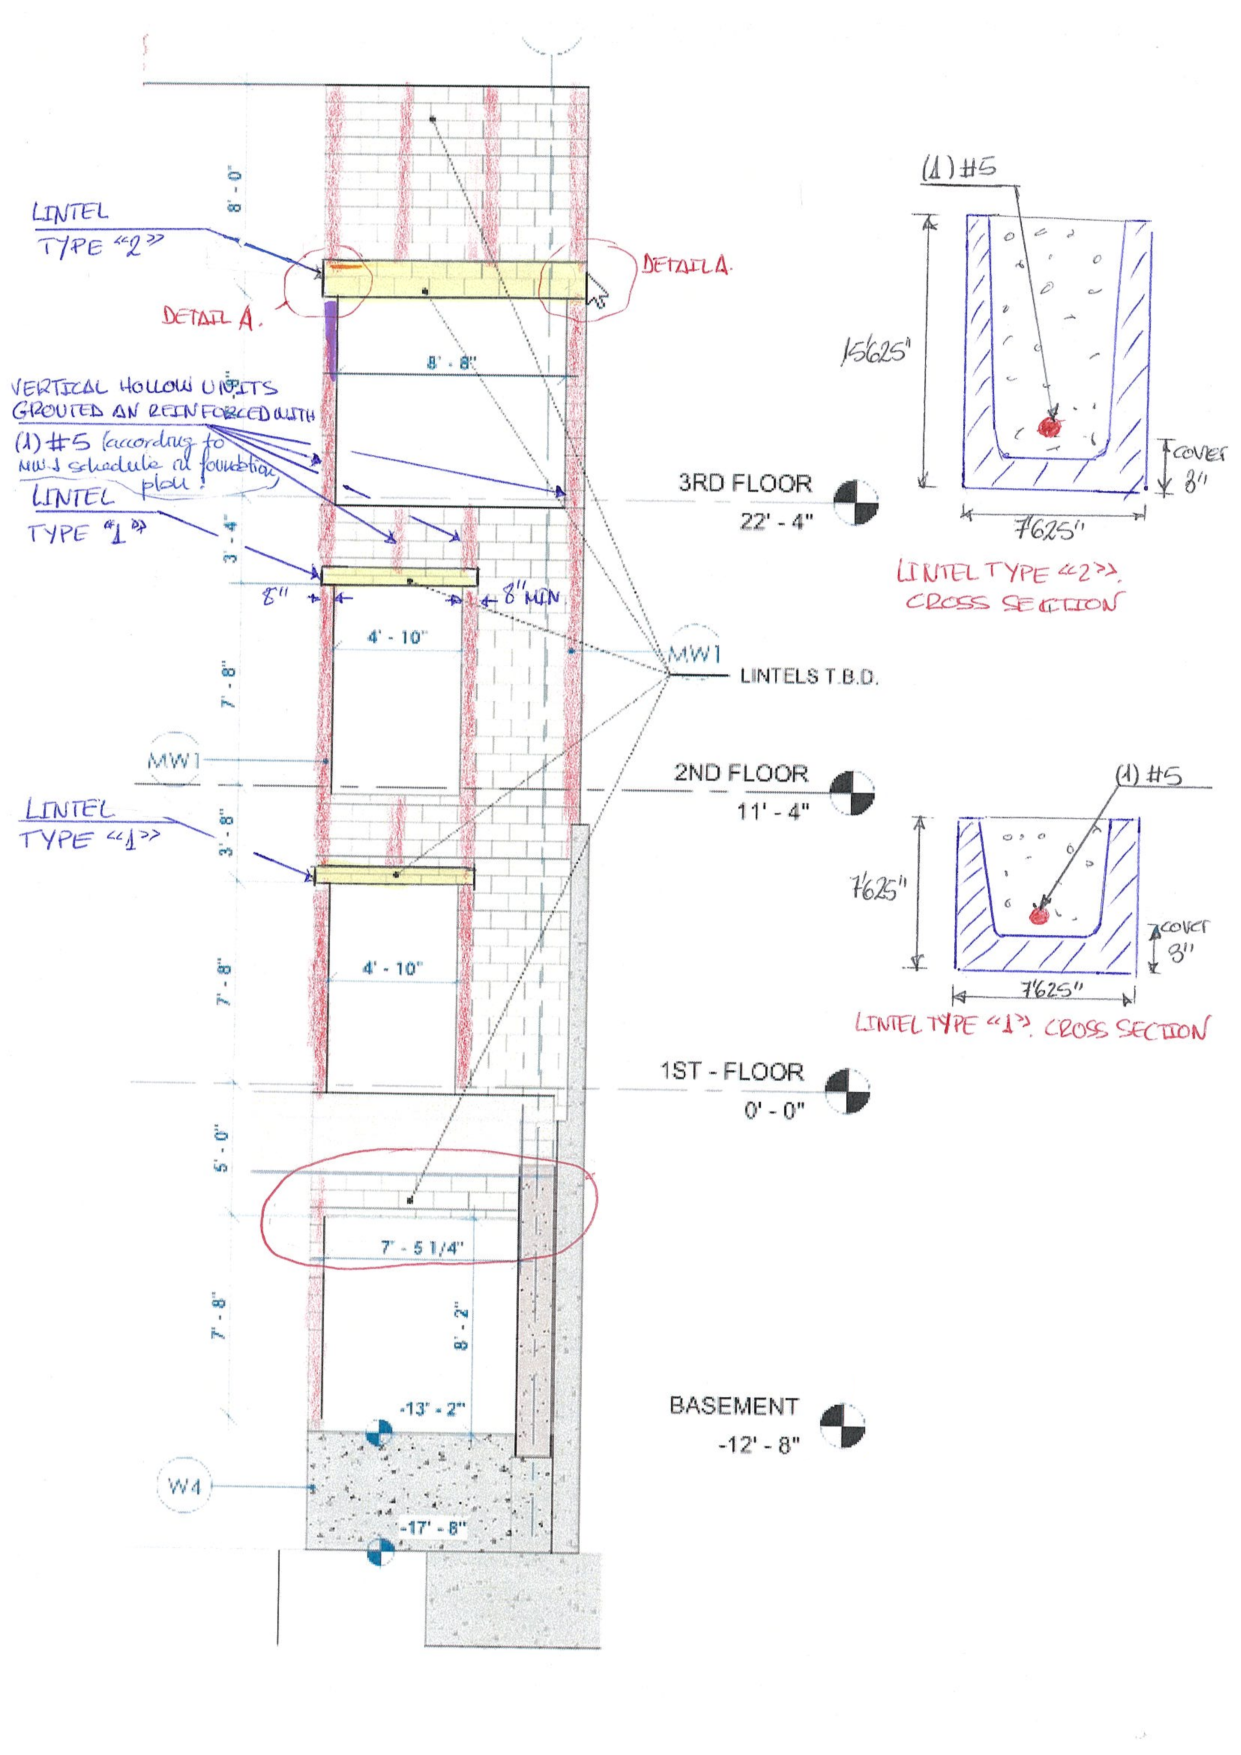
\includegraphics[width=120mm]{results_lintels/lintels_figures/elevator_lintels-1.pdf}
  \end{center}
  \caption{Elevator lintels}\label{elevator_lintels.pdf}
\end{figure}

\subsection{Lintel 3rd and 2nd floor}
\subsubsection{Geometry data}
Clear span=  4 feet 10 inches \\
Bearing length (at each extremity)=  21/32 inches \\
Height of masonry above the opening=  3 and 11/32 inches \\
Mmax=  1910.65 lb-ft = 22927.80  lb-in \\
Vmax=  1389.56 lb \\
\subsubsection{Load data}
Lintel self-weight=  59  $\frac{lb}{ft}$ \\
Wall self weight=  47 $\frac{lb}{ft^2}$ \\
Superimposed dead uniform load=  64.17 $\frac{lb}{ft}$ \\
Live uniform load=  128.33 $\frac{lb}{ft}$ \\
Snow uniform load=  0 $\frac{lb}{ft}$ \\
\vspace{0.25 cm}
\subsubsection{Check for arching action}
Effective span l=  5 feet 5 and 1 inches \\
Height of masonry required above the lintel for arching action to occur=  3 and 13/32 inches \\
Arching action occurs (not considered conservatively) \\
\subsubsection{Check concrete masonry lintel - strenght design}
Maximum bending moment due to lintel self weigth=  223.09 lb-ft \\
Maximum bending moment due to wall self weigth=  479.47 lb-ft \\
Maximum bending moment due to superimposed dead load=  242.63 lb-ft \\
Maximum bending moment due to live load=  485.26 lb-ft \\
Maximum bending moment due to snow load=  0.0 lb-ft \\
Maximum bending moment ULS01=  1323.27 lb-ft \\
Maximum bending moment ULS02=  1910.65 lb-ft \\
Maximum bending moment ULS03=  1376.86 lb-ft \\
Maximum bending moment=  1910.65 lb-ft \\
Bending moment provided= 5165.00 lb-ft (see fig \ref{8x8}) \\
Maximum shear force due to lintel self weigth=  162.25 lb \\
Maximum shear force due to wall self weigth=  348.71 lb \\
Maximum shear force due to superimposed dead load=  176.46 lb \\
Maximum shear force due to live load=  352.92 lb \\
Maximum shear force due to snow load=  0.0 lb \\
Maximum shear force ULS01=  962.38 lb \\
Maximum shear force ULS02=  1389.56 lb \\
Maximum shear force ULS03=  1001.36 lb \\
Maximum shear force=  1389.56 lb \\
Shear force provided= 5232.00 lb (see fig \ref{8x8}) \\

%% \begin{table}[h]
%%   \begin{center}
%%    \caption{\textbf{Allowable Shear and Moment for Nominal 8 x 8 in. Concrete Masonry Lintels}} \label{8x8}
%%    \begin{tabular}{llllllllll}
%%       Steel & No. & & & & Bottom Cover (in.) & & & \\
%%       \arrayrulecolor{gray}\hline
%%       Size & of & 1.5 & & 2 & & 2.5 & & 3 & \\
%%       \arrayrulecolor{gray}\hline
%%       (No.) & Bars & $V_{all}$ & $M_{all}$ & $V_{all}$ & $M_{all}$ & $V_{all}$ & $M_{all}$ & $V_{all}$ & $M_{all}$ \\
%%       & & lb & in.-lb & lb & in.-lb & lb & in.-lb & lb & in.-lb \\
%%       \hlineB{2}
%%       4 & 1 & 1734 & 20464 & 1587 & 17651 & 1439 & 14997 & 1292 & 12509 \\
%%       \arrayrulecolor{gray}\hline
%%       5 & 1 & 1716 & 23176 & 1568 & 19898 & 1421 & 16816 & 1273 & 13938 \\
%%       \arrayrulecolor{gray}\hline
%%       6 & 1 & 1698 & 25219 & 1550 & 21557 & 1402 & 18125 & 1255 & 14933 \\
%%       \arrayrulecolor{gray}\hline
%%       4 & 2 & 1734 & 25468 & 1587 & 21866 & 1439 & 18481 & 1292 & 15323 \\
%%       \arrayrulecolor{gray}\hline
%%       5 & 2 & 1716 & 28142 & 1568 & 24036 & 1421 & 20194 & 1273 & 16628 \\
%%       \arrayrulecolor{gray}\hline
%%       6 & 2 & 1698 & 29973 & 1550 & 25478 & 1402 & 21289 & 1255 & 17418 \\
%%       \hlineB{2}
%%   \end{tabular}
%%   \end{center}
%% \end{table}
\begin{figure}
  \begin{center}
  \includegraphics[width=120mm]{results_lintels/lintels_figures/blocks_8_8}
  \end{center}
  \caption{Design shear and moment capacity for nominal 8 x 8 in. concrete masonry lintels}\label{8x8}
\end{figure}


\subsubsection{Check lintel deflection}
Modulus of elasticity E=  194400000.0  psf \\
Moment of inertia I=$  0.0135847972744$  $ft^4 $
$\Delta_{max,dead} =$  0.01353  in \\
$\Delta_{max,live} =$  0.00695  in \\
$\Delta_{max,snow} =$  0.0  in \\
$\Delta_{max} =$  0.02048  in \\
$\Delta_{max,allowed} =$  0.11  in \\
$\Delta_{max} =$  0.02048  < $\Delta_{max,allowed} =$  0.11  ok \\
